\addtocontents{toc}{\protect\setcounter{tocdepth}{0}}

\chapter{Implementation}
\label{appendix:implementation}


This section describes how we implemented adaptive recommenders.
This is a short description of the most important features and considerations
made when implementing the system.
While quite specific and not important to the viability of 
\emph{adaptive recommenders} in itself,
this should give a short introduction to how this technique can be put into practice.

\section{Libraries}

\begin{figure}[t]
  \begin{center}
    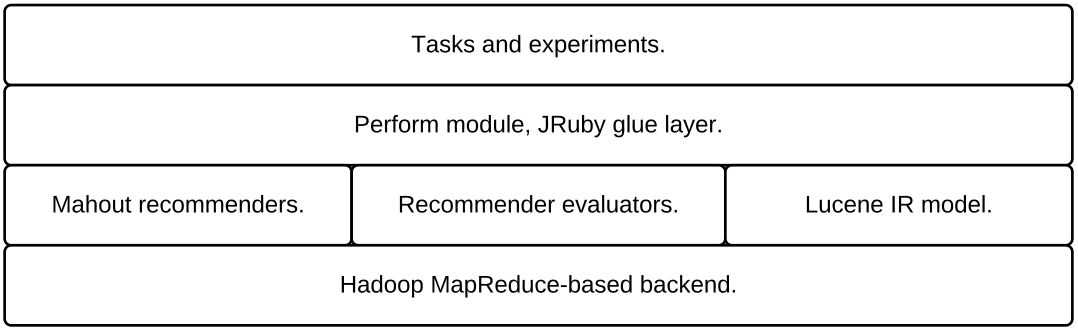
\includegraphics[
      width=1.0\textwidth]{../graphics/diagram-app-layers}
    \caption[Library Layers]{
      Library layers:
      Tasks and experiments are performed by the custom JRuby glue layer.
      Recommenders are created by the Mahout machine learning library.
      IR models are based on the Lucene search engine library.
      Recommender evaluators are created in Ruby.
      Each of the intermediary layers are built on the Hadoop
      MapReduce framework for efficient parallel computation. 
    }
  \label{fig:library-layers}
  \end{center}
\end{figure}

Naturally, the most important part of the implementations are the recommender systems.
These are used for the basic ratings predictions, and to 
create the adaptive aggregation by predicting the accuracy of other recommenders.
At the same time, these different recommenders need to have the same
interface for training and testing, regardless of which context
each experiment places them into.
Our implementation makes use of a number of external libraries,
as seen in Figure \ref{fig:library-layers}

To quickly get a large number of recommenders up and running,
the system was linked with the \emph{Apache Mahout machine learning library}
(See Appendix \ref{appendix:resources}). 
Mahout provides a number of machine learning
algorithms, amongst which a set of recommender systems.
Examples include SVD- and kNN-based recommenders,
baseline recommenders, a Slope One recommender,
cluster-based recommenders,
and various generic recommenders for mixing different 
similarity and neighborhood measures.
Mahout is a young project, launched in 2008, 
but was found to be quite mature and feature-rich
in our experience.

Mahout is build on top of \emph{Apache Hadoop},
a system for creating scalable and distributed data processing systems 
(See Appendix \ref{appendix:resources}).
This is important to the performance of our system.
As mentioned, a lot of the operations performed in layering recommenders
are independent and lend themselves well to parallelization.
By building on Hadoop, each of our recommenders come implemented in a 
proper MapReduce framework for parallel computation (as explained in \citet[p75]{Manning2008}).
Each of the basic recommenders and adaptive aggregators can then be modeled at the same time,
making the most out of whatever hardware is present.

For our IR tasks, we chose to build on another library.
\emph{Apache Lucene} (See Appendix \ref{appendix:resources}) is an open-source search engine, also built on top of Hadoop,
gaining the same performance wins as Mahout.
Lucene provides powerful methods for creating indexes of items, and for querying these indexes.

Mahout, Lucene and Hadoop are all written in the Java Programming Language,
and runs on the Java Virtual Machine (JVM).
To facilitate rapid prototyping, the Ruby scripting language was chosen as a "glue" language,
for interfacing with the libraries. 
By using the JRuby implementation of Ruby, Java libraries can be imported directly
into the language, allowing us to use Mahout and Hadoop almost as if they were written in the same language.
The use of Ruby allowed us to quickly develop different combinations of recommenders and
perform varying experiments in a short amount of time.

\section{Task Structure}

\begin{figure}[t]
  \begin{center}
    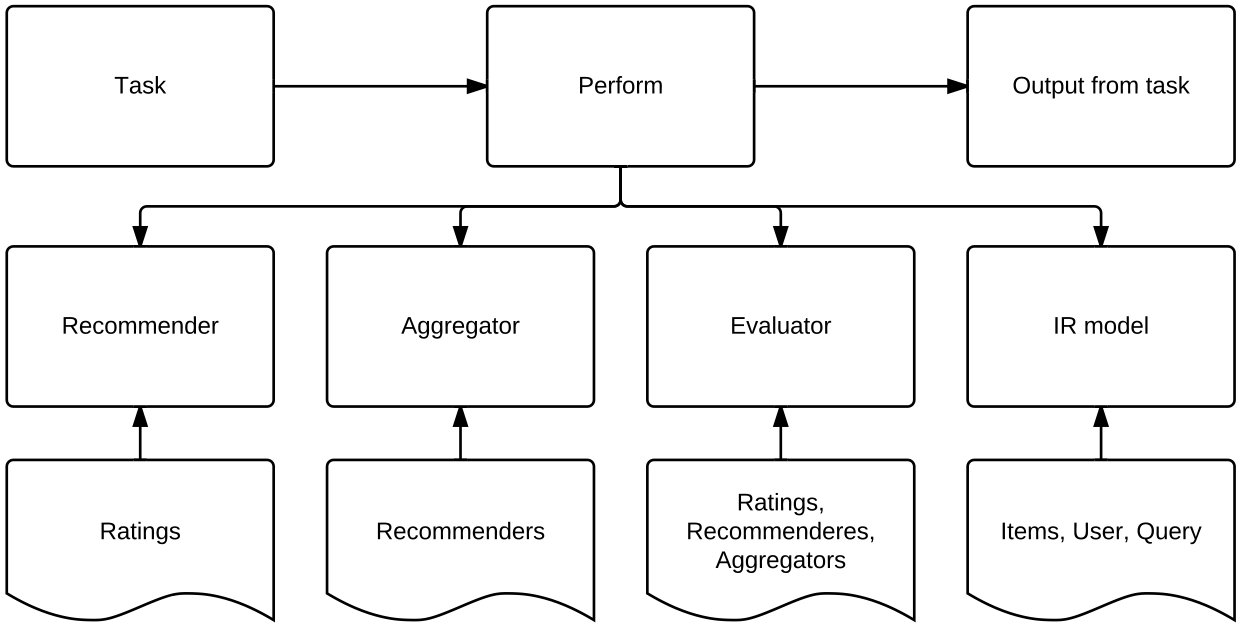
\includegraphics[
      width=1.0\textwidth]{../graphics/diagram-task}
    \caption[Task Structure Diagram]{
      Task structure diagram:
      A task (instantiated configuration) is passed to the perform module.
      This module creates a number of modules:
      recommenders, aggregators, evaluators and information retrieval models.
      Each module takes a set of inputs (bottom row), 
      which are specified by the current task.
      These modules are then used as needed by each experiment.
    }
  \label{fig:uml}
  \end{center}
\end{figure}

In order to facilitate rapid prototyping,
our system is built around a few core concepts that can
be used together in different ways.
Everything the system does is considered a \emph{task}.
A task is a collection of settings and directives
and serves as instantiated configurations for the system.
Tasks are created beforehand, and fed into the system,
which carries them out.
Tasks specify what the system should do,
which dataset should be used, and other options.
See Figure \ref{fig:uml} for the overall structure.

The most important task is creating a recommender.
As recommenders are used both for the standard rating predictions,
and for the adaptive error estimations, creating recommenders
are the most common and important task of this system.
Another important task is creating evaluators.
An evaluator takes a set of recommenders as input,
tests them against the dataset specified in the task,
and returns the results of the evaluation.


\section{Modeling \emph{\&} Prediction}

The modeling phase consists of running our modeling algorithms and storing the resulting models.
A task is created for each of the basic recommenders, and for each of the adaptive recommenders.
If this is a rank aggregation scenario, an IR model is also created, based on the data
specified by the current task.
As mentioned, this is an offline approach, so that the models can be computed and recomputed,
independent of making any actual predictions.

Our experiments required us to measure the performance of each
recommender, and the adaptive recommender, for every combination of 
a user and an item.
In order to perform these experiments, an \emph{evaluator} module was built.
As both the standard recommenders and the adaptive recommender system presents the same 
interface, the evaluators simply takes a set of recommenders as input, 
and measures their accuracy across the dataset specified by the current task.

This prediction phase, where each user is compared to every unrated item,
is not comparable to the prediction phase of a real-world system
based on adaptive recommenders. In a real world application of this technique,
a prediction is made whenever a user's actions requires it,
e.g. when we need to know what a user will think of an item.

This is where the $\mathrm{MapReduce}$ operations previously mentioned come into play.
Each of the basic recommenders, and each of the adaptive recommenders can be applied in parallel.
The basic recommenders are applied through a $\mathrm{map}$ operation, where the current user and item (the input)
is given to each modeling method. These methods return a number of scalar predictions.
The next step is the $\mathrm{reduce}$ operation, which is the adaptive layer.
Here, the scalar predictions are reduced to one prediction by computing weights
based on probable accuracy.
These computations can of course be cached, if certain combinations of users and items
often need predictions.

As mentioned, none of these aspects have any bearing on the viability of adaptive recommenders.
However, as this does provide an example of how to implement such a system. 
See Appendix \ref{appendix:resources} for links to other resources. 


\section{Example Task}

This section gives an example of an experiment run through our system.
In this experiment, we wish to create our adaptive recommender
and test it on the MovieLens dataset.
The code is written in JRuby, just as it is in the implementation.

First, we create our tasks and run these tasks to create the recommenders.
We then create an evaluator to test our resulting adaptive recommender.
The resulting RMSE values are output to the screen
(see Listing \ref{code:example})

\begin{implementation}{code:example}{Example code showing a test of adaptive recommenders.}
d_m = "movielens/base/1"
d_t = "movielens/test/1"

# Standard recommenders
recommender_tasks = {
  knn:        Task.new(recommender: :generic_user, dataset: d_m),
  item_avg:   Task.new(recommender: :item_average, dataset: d_m),
  slope_one:  Task.new(recommender: :slope_one, dataset: d_m),
  baseline:   Task.new(recommender: :item_user_average, dataset: d_m),
  cosine:     Task.new(recommender: :generic_item, dataset: d_m) 
}
rs = Perform.perform(recommender_tasks)

# Aggregate recommenders
aggregate_tasks = {
  average: Task.new(recommender: :aggregate, method: :average, recommenders: rs),
  median:  Task.new(recommender: :aggregate, method: :median,  recommenders: rs)
}
aggregate_recommenders = Perform.perform(aggregate_tasks)

# Adaptive recommender
adaptive_task = Task.new(recommender: :adaptive, recommenders: rs)
adaptive_recommender = Perform.perform(adaptive_task)

# Merge all recommenders
all = rs.merge(aggregate_recommenders).merge(adaptive_recommender)

# Evaluation
evaluator_task = Task.new(mission: :rmse_evaluator, recommenders: all, dataset: d_t)
evaluator = Perform.perform(evaluator_task)

# Run experiment
result = evaluator.evaluate
Log.evaluation(result)
\end{implementation}


\section{Running the Experiments}

To tun the experiments, a few libraries must be installed. 
First, JRuby must be available (see links in Appendix \ref{appendix:resources}).
This has to be a version capable of running code conformant to Ruby version 1.9 (e.g. JRuby 1.6).
The \emph{rake} library should also be installed, as it is used to start and run each experiment.

To get the system up and running in a Posix-based environment, 
the following steps should be run.
The \textsf{\$} refers to the operator in a terminal window.
All commands should be run from the top-level folder of the implementation source code.

\begin{enumerate*}
  \item Install JRuby (version >= 1.6) from their website.
  \item Install rake: \textsf{\$ jruby -S gem install rake}
  \item Run each experiment: \textsf{jruby -S rake e1}
  \item Substitute \textsf{e1} with \textsf{e2} or \textsf{e3} to run each experiment.
\end{enumerate*}

On some systems, the JRuby VM might run out of memory due to its low default setting.
To manually allow more memory to be used, the following command
can be substituted in when running each experiment:

{
\footnotesize
\begin{verbatim}
jruby --1.9 -J-Xmn512m -J-Xms2048m -J-Xmx2048m experiment1.rb
\end{verbatim}
}

The first parameter specifies that this application should be run with version 1.9 of the Ruby language specification.
The second specifies the minimum garbage collection memory size.
The two following gives the minimum and maximum heap memory size.
The last part of this command is the file that should be run.
Each experiment has its own file.


\chapter{Resources}
\label{appendix:resources}

This appendix gives pointers to additional resources mentioned throughout this thesis.

\paragraph{Implementation Code}
The code for the implementation outlined in Appendix \ref{appendix:implementation} is available online.
It resides in version control at 
\url{github.com/olav/thesis/tree/master/code}.

The implementation is built on three open-source libraries from the
Apache Project\footnote{See \url{www.apache.org/} --- accessed 19/5/2011}:
The Hadoop distributed computing library\footnote{See \url{hadoop.apache.org/} --- accessed 19/5/2011},
the Mahout machine learning library\footnote{See \url{mahout.apache.org/} --- accessed 19/5/2011},
and the Lucene information retrieval library\footnote{See \url{lucene.apache.org/} --- accessed 19/5/2011}.

Specific versions of these libraries are bundled together with
the source code as JAR-files, that run on the JVM.
Note that these libraries are released under their own terms,
namely the Apache License\footnote{
See \url{www.apache.org/licenses/} --- accessed 19/5/2011}.
The repository also includes the glue-code, written in ruby and run on the JRuby\footnote{
See \url{www.jruby.org/} --- accessed 09/05/2011} interpreter.

\paragraph{Previous Work}
Parts of this thesis is based on a previous work in the same field:
\cite{Bjorkoy2010d}. This paper is avaiable from
\url{github.com/olav/papers/raw/master/user.modeling.on.the.web.pdf}.

\paragraph{Document Details}
This thesis is written in the LaTeX document preparation system.
It is based on a LaTeX-template called Memoir\footnote{
See \url{www.ctan.org/tex-archive/macros/latex/contrib/memoir/} --- accessed 19/5/2011.}.
Most of the figures and graphs are made with the TikZ and PGF graphics libraries\footnote{
See \url{www.texample.net/tikz/} --- accessed 23.05.2011}.

The entire source code for this document can be found at 
\url{github.com/olav/thesis/tree/master/thesis}.
The most current PDF-version is also available from this site.
%The source code for the implementation, this document, and the thesis itself
%is available under a Creative Commons BY 3.0 license\footnote{
%See \url{creativecommons.org/licenses/by/3.0/}}.
%Anyone is free to share, copy, distribute or transmit this work,
%or adapt it for any purpose,
%as long as the work is attributed to its author.
For citation purposes, use the following BibTex entry:

{
\footnotesize
\begin{verbatim}
@mastersthesis{Bjørkøy2011,
  address = {Trondheim, Norway},
  author  = {Bjørkøy, Olav},
  school  = {NTNU},
  year    = {2011},
  title   = {{Adaptive Recommenders: 
              Personalized Prediction Aggregation
              Through Accuracy Estimation}}
} 
\end{verbatim}
}

